\section{Utilizzo di Butterfly}\label{utilizzo}


\subsection{Webhooks} % Boh, da vedere se mettere qui o in configurazione

Butterfly ha lo scopo di restare in ascolto degli \gloss{webhook} provenienti da GitLab e Redmine.
Per fare ciò, è necessario configurare degli webhook dalle applicazioni e progetti interessati e aggiungere
la porta dove il \gloss{Producer} di quell'applicazione è in ascolto.

\subsection{Redmine}
TODO

\subsection{GitLab}

Per aggiungere un webhook relativo a un progetto su GitLab, andare sulle impostazioni di quel progetto:

\begin{center}
    \texttt{Settings > Integrations}
\end{center}

Aggiungere gli eventi di interesse (attenzione: Butterfly non supporta tutti gli eventi) e mettere nel URL
l'indirizzo su cui il Producer GitLab è in ascolto (di default la porta è 5003, è possibile cambiare questa impostazione
nel file \texttt{producer/gitlab/config.json}): % TODO: JSON cambiabile da rancher? Meglio prendere la variabile d'ambiente?

\begin{center}
    \texttt{http://alpha6-rancher-node.imolab.it:5003}
\end{center}

\begin{figure}[H]
    \centering
    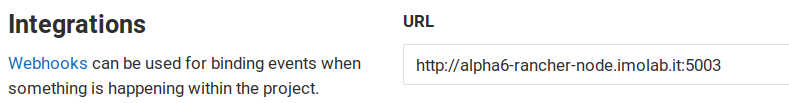
\includegraphics[width=\textwidth]{img/webhook-gitlab.png}\\
    \caption[Webhook, GitLab]{Inserimento URL per configurare un webhook su un progetto (GitLab)}
\end{figure}


\subsubsection{Eventi supportati}
Segue la lista degli eventi supportati dal Producer GitLab:
\begin{itemize}
    \item Push events
    \item Comments
    \item Issues events
\end{itemize}

% Resto delle attività utile all'amministratore che configura l'applicazione

\subsection{Gestore Personale}

\subsubsection{Iscrizione a Butterfly}

\subsubsection{Modifica preferenze}

\subsubsection{Inserimento giorni di indisponibilità}

\subsubsection{Aggiunta progetti e priorità}

\subsubsection{Disiscrizione}

\subsection{Configurazione piattaforma di messaggistica}

\subsubsection{Email}

Per ricevere i messaggi di Butterfly tramite e-mail, è sufficiente fornire tramite l'interfaccia del Gestore Personale l'e-mail sulla
quale si vuole ricevere la notifica.

\subsubsection{Telegram}

Per ricevere le notifiche via Telegram, è necessario fare un passaggio addizionale. Va fornita l'autorizzazione al bot per poter inviare messaggi
agli utenti. Il bot è raggiungibile al seguente link:
\begin{center}
    \url{http://t.me/ConsumerSbot}
\end{center}

Dare il comando \texttt{/start} per dare l'autorizzazione di inoltro dei messaggi al bot.
Sarà poi necessario aggiungere tramite l'interfaccia del Gestore Personale il proprio account Telegram.
